%%%%%%%%%%%%%%%%%%%%%%%%%%%%%%%%%%%%%%%%%%%%%%%%%%%%%%%%%%%%%%%%%%%%%%%% NEED the picture attached inside the HotelTraffic.zip file to compile
%%%%%%%%%%%%%%%%%%%%%%%%%%%%%%%%%%%%%%%%%%%%%%%%%%%%%%%%%%%%%%%%%%%%%%%% Name of Picture HotelTraffic.png
\documentclass[a4paper]{article}
\usepackage{a4wide}
\usepackage{longtable}
\usepackage{graphicx}
\usepackage{verbatim}
\usepackage{color}
\usepackage[normalem]{ulem}
%% gives strikeout capability with \sout{}
%Gummi|063|=)
\title{\textbf{Assignment 2 COMP2111 13s1\\Traffic Around the Hotel}}
\author{Jiashu Chen\\
}

\date{Revision 1.3 of Date: MAY/12/2013 19:20}


\begin{document}
\thispagestyle{empty}
\maketitle
\tableofcontents
\newpage
\setcounter{page}{1}
%%%%%%%%%%%%%%%%%%%%%%%%%%%%%%%%%%%%%%%%%%%%%%%%%%%%%%%%%%%%%%%%%%%%
\section{Introduction}

\indent\indent The project is designed for the local council to fix the traffic light management system that is currently used around the Hotel.

The aim is to design a system which will guarantee the following properties:
\begin{description}
\item [Safety:] Traffic is safe around the hotel, that is, no two conflicting lights are green at the same time. In fact, a stronger form is required: before one of set of conflicting lights can turn green, all the others need to be red.
\item [Fairness:] Traffic management aspires to be fair in the sense that, if a light has been requested to become green (by a pedestrian pushing a button or by a car stopping on the induction coil), then no conflicting light can become green twice without becoming green.1
\item [Flow:] If a light has been requested to become green (by a pedestrian pushing a button or by a car stopping on the induction coil), then it will eventually become green.
\end{description}

\section{Problem Statement: Entity Representation and Requirements}
\subsection{Hotel Structure Representation}

\begin{figure}[h!]
  \begin{center}
  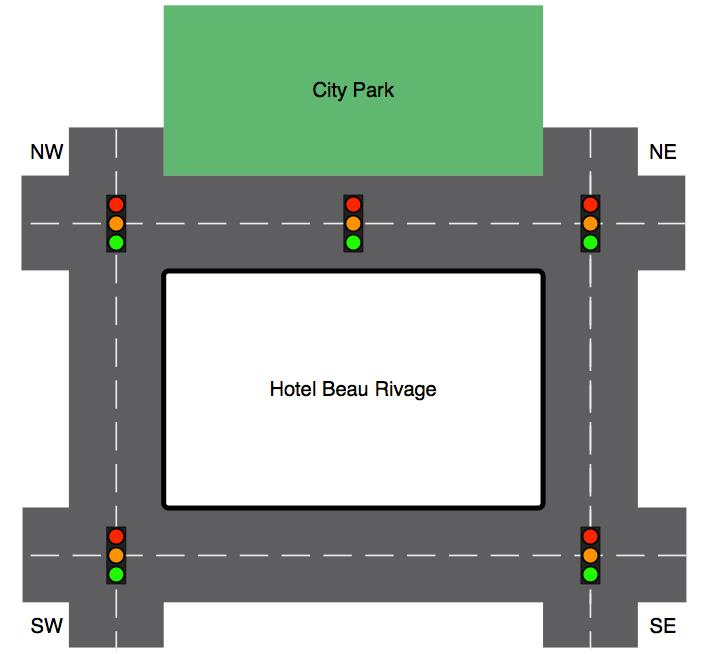
\includegraphics[width=0.7\textwidth]{HotelTraffic.jpg}
  \caption{Hotel Structure}
  \end{center}
\end{figure}

\newpage
\noindent As shown in the diagram the structure representation of the traffic facilities around the hotel will be the following:\\

\begin{longtable}{|l|p{2.4cm}|p{4.1cm}|p{4.5cm}|}
  \caption{Table of Hotel Traffic Entity Representation}\\
  \hline
  \multicolumn{1}{|c|}{\textbf{Type}}  &
  \multicolumn{1}{|c|}{\textbf{Name}} &
  \multicolumn{1}{|c|}{\textbf{Level First Introduced}} &
  \textbf{Short Description}\\
  \hline\hline
  \endfirsthead
  \caption[]{Table of Hotel Traffic Representation \textit{Continued}}\\
  \hline
  \multicolumn{1}{|c|}{\textbf{Type}}  &
  \multicolumn{1}{|c|}{\textbf{Name}} &
  \multicolumn{1}{|c|}{\textbf{Level First Introduced}} &
  \textbf{Short Description}\\
  \hline\hline
  \endhead
  \hline
  \multicolumn{4}{r}{\textit{continued on next page\ldots}}\\
  \endfoot
  \hline
  \endlastfoot
   Intersection & NW & Abstract Model &The conjunction on the top-left of the diagram.\\
   \hline
   Intersection & SW & Abstract Model &The conjunction on the bottom-left of the diagram.\\
   \hline
    Intersection & NE & Abstract Model &The conjunction on the top-right of the diagram.\\
   \hline
   Intersection & SE & Abstract Model &The conjunction on the bottom-right of the diagram\\
   \hline
   Intersection & PARK & Abstract Model & The conjunction on the center-top of the diagram.\\
   \hline
   Direction & NORTHSOUTH & Abstract Model & The "vertical" direction of the diagram\\
   \hline
   Direction & EASTWEST & Abstract Model & The "horizontal" direction of the diagram\\
   \hline
   Relation & Road & Emergency & A relation which tell every other intersection include itself, which are on the same road with this intersection.\linebreak\linebreak For example, if input (NW, NORTHSOUTH) the set of intersections that mapped to this ordered pair, will be {NW, SW}\\
   \hline
   COLOR & {\color{red}RED} & Abstract Model & The {\color{red}red} color.\\
   \hline
    COLOR & {\color{green}GREEN} & Abstract Model & The {\color{green}green} color.\\
   \hline
    COLOR & {\color{yellow}AMBER} & Abstract Model & The {\color{yellow}amber} color.\\
   \hline
   Relation & nextColor & Abstract Model & Tell how the color cycle should change, for example the nextColor of RED should be GREEN, nextColor of GREEN should AMBER, nextColor of AMBER should be RED.
\end{longtable}

\subsubsection{Overall Implementation Strategy}

\indent\indent In order to simplify the problem, the system implement separate events for different condition, e.g. there is a event, which will change the traffic light for intersection, which has no sensors triggered, and another event which change color for intersections, which has sensor triggered.

\subsection{Task 1: Abstract}
\subsubsection{Requirements}
\begin{center}
\begin{tabular}{|p{3.5cm}|p{10cm}|}
\hline
\color{blue}{Requirements} & \color{blue}{Function}\\
\hline
  Change color of lights & The system should be change color of traffic light and pedestrian light of each direction and intersection.\\
  \hline
  Safety Feature 1&  For every intersection, if the traffic light on direction one is GREEN or AMBER, it implies the traffic light on the other direction must be RED.\\
  \hline
   Safety Feature 2 & For every intersection, if the traffic light on direction one is GREEN or AMBER, it implies the pedestrian light on the other direction must be RED.\\
  \hline
  Safety Feature 3 & For every intersection, and for both the traffic light and pedestrian light, the light on two different direction can only be RED at the same time.\\
  \hline
  Safety Feature 4 & For every intersection, pedestrian light can only turn GREEN, if the traffic light on the same direction is GREEN. \\
  \hline
\end{tabular}
\end{center}
\subsubsection{Implementation Strategy}

\indent\indent For the ease of modeling, the system treat the Intersection PARK, which doesn't have traffic light on the NORTHSOUTH direction, same as every other direction.
=
\indent This implies that the whole process for change of color for pedestrian light and traffic can be modeled with two events. since every intersection are treated the same.

\indent For the purpose of Emergency, the system also have a set of events which will initiate a safe condition for the traffic.

\begin{center}
\begin{tabular}{|p{3.5cm}|p{10cm}|}
\hline
\color{blue}{Events} & \color{blue}{Usage}\\
\hline
  changeTrafficCycle & The event which will change the color of all intersection. The event does the same thing as all 3 events:\begin{itemize}
  \item changeTrafficToRED
  \item changeTrafficToAMBER
  \item changeTrafficToGREEN
\end{itemize} combined together.\\
\hline
  changeTrafficToRED & Set the color of light(traffic) to RED, A separate event used to ensure the ease of modeling in later refinements when sensors are added.\\
  \hline
  changeTrafficToAMBER & Set the light(traffic) to AMBER, A separate event used to ensure the ease of modeling in later refinements when sensors are added.\\
  \hline
  changeTrafficToGREEN & Set the light(traffic) to GREEN, A separate event used to ensure the ease of modeling in later refinements when sensors are added.\\
  \hline
  changePedToGreen & Set the light(pedestrian) to GREEN.\\
  \hline
  changePedToRed & Set the light(pedestrian) to GREEN.\\
  \hline
  roadToGreen & Set the light(traffic) on the road to GREEN, used for later emergency refinement.\\
  \hline
  roadToOPPOSITERed & Set all lights to RED, used for later emergency refinement.\\
  \hline
\end{tabular}
\end{center}
\newpage
\subsection{Task 2: Add Sensor}
\subsubsection{Requirements}
\begin{center}
\begin{tabular}{|p{3.5cm}|p{10cm}|}
\hline
\color{blue}{Requirements} & \color{blue}{Function}\\
\hline
  Detect Sensor & The system should be able to detect if a sensor is triggered, and register status accordingly.\\
  \hline
  Fairness Feature 1& Sensor can not be trigger if the light on the direction triggered at a intersection is not RED.\\
  \hline
  Fairness Feature 2 & If a intersection has a sensor triggered, then the direction at the intersection become GREEN mush be the same as the direction triggered.\\
  \hline
  Fairness Feature 3 & Sensor can only be triggered once. \linebreak This implies once a sensor is triggered it can't be triggered again until the color on this intersection becomes GREEN.\\
  \hline
   Fairness Feature 4 & Sensor only valid for one time. \linebreak This implies once the light become GREEN, the sensor must be set to be not triggered state.\\
  \hline
\end{tabular}
\end{center}
\subsubsection{Implementation}
\begin{center}
\begin{tabular}{|p{3.6cm}|p{10cm}|}
\hline
\color{blue}{Event} & \color{blue}{Usage}\\
\hline
  changeTrafficCycle & Used when trigger is not set.\\
  \hline
  changeTrafficToRED & Used when trigger is set.\\
  \hline
  changeTrafficToAMBER & Used when triggered is set.\\
  \hline
  changeTrafficToGREEN & Used when triggered is set.\\
  \hline
  changePedToGreen & Used both when triggered is set and not set.\\
  \hline
  changePedToRed & Used both when triggered is set and not set.\\
  \hline
  roadToGreen & No further change at this level.\\
  \hline
  roadToOPPOSITERed & No further change at this level.\\
  \hline
  triggerTrafficCoil & Trigger the traffic coil on a direction at a intersection.\\
  \hline
  triggerPedSensor & Trigger the pedestrian sensor on a direction at a intersection.\\
\hline
\end{tabular}
\end{center}
\indent\indent At this level, when sensors on both direction at a intersection the fairness of FIRST PRESS FIRST TURN TO GREEN is not guaranteed to happen.

Also this level weak fairness is required for events, since the B-Language can't guarantee the flow of system, it is not clearly indicated. However the flow of system is improved by setting a more deterministic model(separate turn traffic light system).

\newpage

\subsection{Task 3: Add Logic}
\subsubsection{Requirements}
\begin{center}
\begin{tabular}{|p{3.5cm}|p{10cm}|}
\hline
\color{blue}{Requirements} & \color{blue}{Function}\\
\hline
  Fairness Feature 1 & This refinement ensure the sensor that is TRIGGERED FIRST will become GREEN FIRST.\\
  \hline
\end{tabular}
\end{center}

\subsubsection{Implementation}
\indent\indent Fairness Feature 1 is ensured by introduce some new variables, which priorities the sensor at each intersection.
\begin{center}
\begin{tabular}{|p{3.6cm}|p{10cm}|}
\hline
\color{blue}{Event} & \color{blue}{Usage}\\
\hline
  changeTrafficCycle & No further change at this level.\\
  \hline
  changeTrafficToRED & No further change at this level.\\
  \hline
  changeTrafficToAMBER & No further change at this level.\\
  \hline
  changeTrafficToGREEN\linebreak PedSingleTrigger & Turn color of the traffic light when there is only one sensor pressed.\\
  \hline
  changeTrafficToGREEN\linebreak PedDoubleTrigger & Turn color of the traffic light on the direction is more prioritized when both direction is pressed.\\
  \hline
  changeTrafficToGREEN\linebreak TrafficSingleTrigger &  Turn color of the traffic light when there is only one sensor pressed.\\
  \hline
  changeTrafficToGREEN\linebreak TrafficDoubleTrigger & Turn color of the traffic light on the direction is more prioritized when both direction is pressed.\\
  \hline
  changePedToGreen & Restore priority\\
  \hline
  changePedToRed & No further change at this level.\\
  \hline
  roadToGreen & No further change at this level.\\
  \hline
  roadToOPPOSITERed & No further change at this level.\\
  \hline
  triggerTrafficCoil\linebreak NoPriorityUpdate & Trigger sensor without change priority at the intersection. In case, the other sensor is pressed, but not yet changed to GREEN.\\
  \hline
  triggerTrafficCoil\linebreak PriorityUpdate & Trigger sensor with priority update.\\
  \hline
  triggerPedSensor\linebreak NoPriorityUpdate & Trigger sensor without change priority at the intersection. In case, the other sensor is pressed, but not yet changed to GREEN.\\
  \hline
  triggerPedSensor\linebreak PriorityUpdate & Trigger sensor with priority update.\\
\hline
\end{tabular}
\end{center}

The system is still lack of one Fairness feature, if traffic light on directionA is triggered, and the pedestrian on the direction opposite directionA is triggered. The SPEC OF THE ASSIGNMENT has not specified which one should be changed first.

In fact, this system can be tricked into situation due to the conflicting priority on two direction at the same intersection to become dysfunctional with respect to the fairness established.

\newpage

\subsection{Task 4: Emergencies}
\subsubsection{Requirements}

\begin{center}
\begin{tabular}{|p{3.5cm}|p{10cm}|}
\hline
\color{blue}{Requirements} & \color{blue}{Function}\\
\hline
 Emergency & Every other event should give way to emergency.\\
 \hline
\end{tabular}
\end{center}


\subsubsection{Implementation}
\begin{center}
\begin{tabular}{|p{3.5cm}|p{10cm}|}
\hline
\color{blue}{Event} & \color{blue}{Usage}\\
\hline
  changeTrafficCycle & Function only when no emergency happen.\\
  \hline
  changeTrafficToRED & Function only when no emergency happen.\\
  \hline
  changeTrafficToAMBER & Function only when no emergency happen.\\
  \hline
  changeTrafficToGREEN\linebreak PedSingleTrigger & Function only when no emergency happen.\\
  \hline
  changeTrafficToGREEN\linebreak PedDoubleTrigger & Function only when no emergency happen.\\
  \hline
  changeTrafficToGREEN\linebreak TrafficSingleTrigger & Function only when no emergency happen.\\
  \hline
  changeTrafficToGREEN\linebreak TrafficDoubleTrigger & Function only when no emergency happen.\\
  \hline
  changePedToGreen & Function only when no emergency happen.\\
  \hline
  changePedToRed & Function only when no emergency happen.\\
  \hline
  triggerTrafficCoil & Function only when no emergency happen.\\
  \hline
  triggerPedSensor & Function only when no emergency happen.\\
  \hline
  InitEmergency & Initiate a safe situation, and set the road ,which is request to be ready for emergency.\\
  \hline
  SetEmergency & Turn every light on the same direction to be green, and shut off the emergency alert.\\
\hline

\end{tabular}
\end{center}
\newpage
\section{Comments: Undischarged POs and Development Related Issue}
\subsection{Task 1: Abstract Model}
\begin{center}
\begin{tabular}{|p{3.5cm}|p{10cm}|}
\hline
\color{blue}{Event} & \color{blue}{PROBLEM}\\
\hline
  changeTrafficCycle & INV3 The problem is same as changeTrafficToGreen.\\
  \hline
  changeTrafficCycle & INV4 The problem is same as changeTrafficToGreen.\\
  \hline
  changeTrafficToGreen & The INV3 should be covered by guard \linebreak trafficLight(intersection \verb+ |-> + otherDirection(direction)) = RED\\
  \hline
  changeTrafficToGreen & The INV4 should be covered by guard \linebreak pedLight(intersection \verb+ |-> + otherDirection(direction)) = RED\\
  \hline
  roadToGreen & The event is a deterministic event, it only fires when under specified situation. The possible reasons of why it is not discharged is:
  \begin{itemize}
  \item System is too big for it to pick up all invariants
  \item Rodin is worrying about the assigned values within the domain or not, this are ensured by the guard.
  \end{itemize}\\
  \hline
\end{tabular}
\end{center}

\subsubsection{Problems Encountered With Rodin Platform}
Rodin is incapable of picking up all problems as the system grows bigger.
For instance, when all of the context file were merged together at the start of the modeling, Rodin failed every implementation, however, after separating them into different context files, they became provable.
During the development, the animator ProB was updated, and after the update it gives file exception errors, when not supposed to. this was fixed by downgrading the system.
\subsection{Lessons Learnt \& Further Development}
\begin{itemize}
\item always make simple context
\item have separate events for different requirements
\item don't update Rodin Platform.
\end{itemize}
\subsubsection{Further Development Strategy}
\indent\indent Implement the Logic flaw that was specified at the end of the AddLogic Section, which was not specified in the SPEC of the assignment.

Use a better strategy to implement the Light representation, Rodin Platform isn't very good at dealing with proofs involve ordered pairs.

\newpage

\appendix
\section{Reference}
\begin{center}
\textbf{Assignment 2 COMP2111 13s1\\
Traffic Around the Hotel\\}
Kai Engelhardt\\
Revision: 1.2 of Date: 2013/04/29 23:59:49
\end{center}
\end{document}
